\chapter{Softwaretechnik}

Zusammenfassung der Vorlesung "`Softwaretechnik 2"' aus dem Wintersemester 2016.\footnote{\url{https://sdqweb.ipd.kit.edu/wiki/Vorlesung_Softwaretechnik_II_WS16/17}}

\section{Einführung}

\section{Gesetzmäßigkeiten}
\begin{itemize}
	\item \textit{Brook's Law}: "`Adding manpower to a late software projcet makes it later."'
	\item \textit{Boehm's Law}: "`Errors are more frequent during requirements and design."'
	\item \textit{Dijkstra 1969}: "`Testing shows the presence, not the absende of bugs."'
	\item (One of) \textit{Lehman's Laws}: "`A system that is used will be changed."'
	\item \textit{Parnas' Law}: "`Only what is hidden can be chaned without risk"' (\(\rightarrow\) Kapselung notwendig)
\end{itemize}



\section{Software-Entwicklungsprozess}

\begin{itemize}
	\item "`Code and Fix"', als Vorgehensmodell unzureichend, da es zu schlecht strukturierten und dokumentierten Programmen führt
	\item Vorgehensmodell: Abstrakte Beschreibung eines Software-Entwicklungsprozesses. Beinhaltet Richtlinien bezüglich Aktivitäten, Rollen und Ergebnissen (Artefakte, Dokumente, etc.)
	\item \textbf{Wasserfallmodell}
	\begin{itemize}
		\item Phasen und Ergebnisse der Phasen
		\begin{enumerate}
			\item Planung: Lastenheft, Projektplan, Kalkulation
			\item Definition: Pflichtenheft, GUI-Beschreibung, eventuell Benutzerhandbuch
			\item Entwurf: Enwurfsdokumente, Modulführer
			\item Implementierung: Komponenten und Dokumentation, Testeinrichtung
			\item Testen
			\item Einsatz und Wartung: "`Fertiges"' System
		\end{enumerate}
		\item Probleme
		\begin{itemize}
			\item Große Softwareprojekte können i.d.R. nicht komplett (auf mehrere Jahre) geplant werden
			\item Abgrenzung der einzelnen Phasen in der Praxis oft unrealistisch
			\item Zu unflexibel bezüglich Änderungen oder Rückschritten
		\end{itemize}
	\end{itemize}
	\item \textbf{V-Modell} \\\\
		\begin{minipage}{\linewidth}
			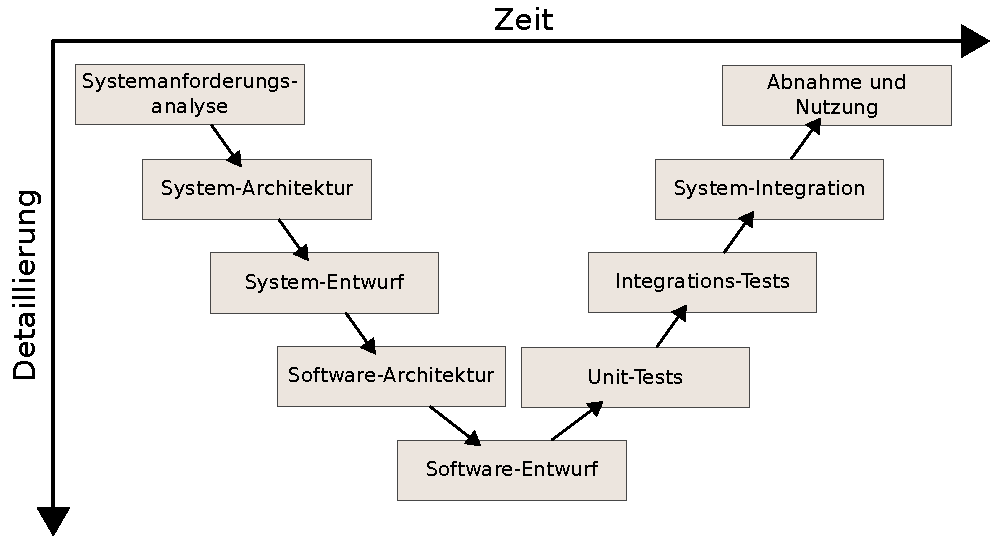
\includegraphics[scale=0.8]{swt2/v-modell.pdf}
		\end{minipage}
\end{itemize}



\section{Agile Entwicklung}

\subsection{Extreme Programming (XP)}
\begin{itemize}
	\item Sammlung aus Werten (Kommunikation, Einfachheit, Feedback, Mut) und Prinzipien (schnelle Lieferung/Feedback, Einfachheit) und Methoden
	\item \textbf{Der Prozess\footnote{\url{http://www.extremeprogramming.org/map/iteration.html}}}\\\\
		\begin{minipage}{\linewidth}
			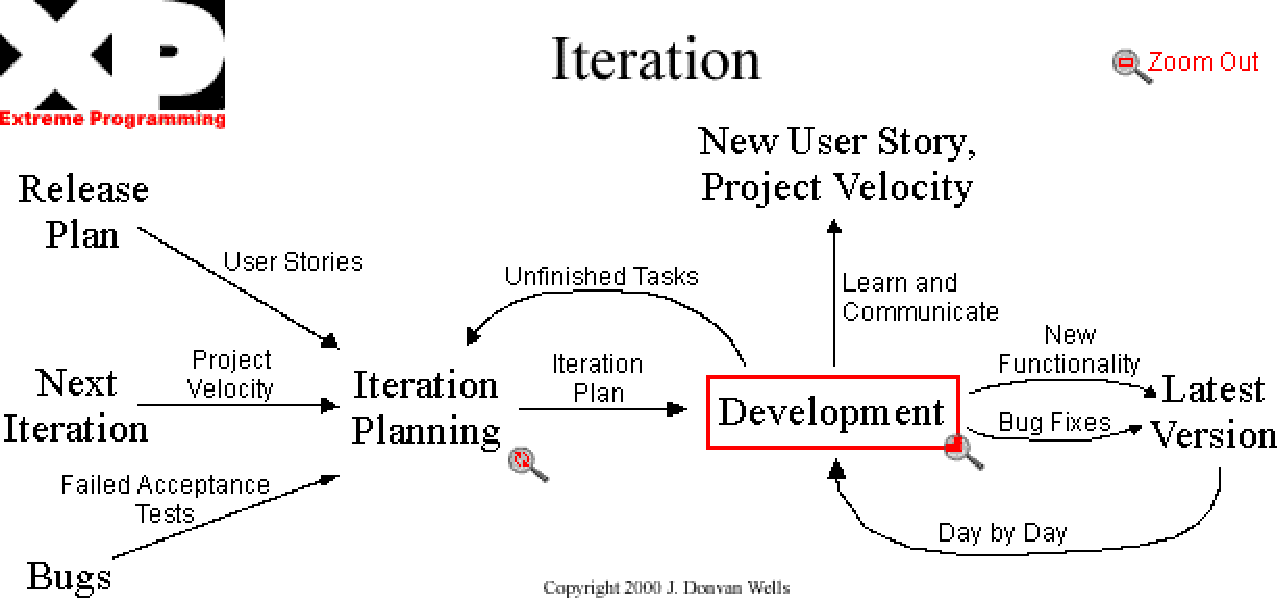
\includegraphics[scale=0.7]{swt2/xp_iteration.pdf}
		\end{minipage}
	\item \textbf{Kritik (allgemein auch an Agile)}
	\begin{itemize}
		\item Schlechte Skalierung bei großen Projekten
		\item Fehlende Dokumentation
		\item Kunden müssen aktiv mitarbeiten
		\item Wirksamkeit mancher Methoden nicht komplett überprüft (beispielsweise Pair-Programming)
	\end{itemize}
\end{itemize}


\subsection{Scrum}
\begin{itemize}
	\item \textbf{Zusammenfassung}
	\begin{itemize}
		\item \textit{Product Owner} erstellt/verwaltet eine priorisierte Liste mit Features, dem \textit{Product Backlog}
		\item Vor jedem \textit{Sprint} entscheidet das \textit{Team} welche Features in diesem \textit{Sprint} umgesetzt werden. Diese werden in den \textit{Sprint Backlog} übernommen
		\item Das \textit{Team} koordiniert die Entwicklung im täglichen \textit{Daily Scrum Meeting}. Der Fortschritt wird in einem Burn-Down-Chart festgehalten
		\item Der \textit{Srum Master} ist für die Kommunikation im \textit{Team} verantwortlich
		\item Während jedem \textit{Sprint} wird ein (möglichst) auslieferungsbereites \textit{Product Increment} erstellt
		\item Letzteres wird vom \textit{Team} im \textit{Sprint Review Meeting} vorgestellt. Anschließend werden im \textit{Retrospective Meeting} mögliche Verbesserungen besprochen
	\end{itemize}
	\item \textbf{Sprints}
	\begin{itemize}
		\item Idealerweise konstante Dauer von höchstens einem Monat
		\item Nach jedem Sprint startet direkt der nächste \(\rightarrow\) der Entwicklungsprozess besteht aus einer Folge von Sprints
		\item Während eines Sprint dürfen keine Änderungen gemacht werden, die das Ziel gefährden oder die Quailität verringern\\\\
		\begin{minipage}{\linewidth}
			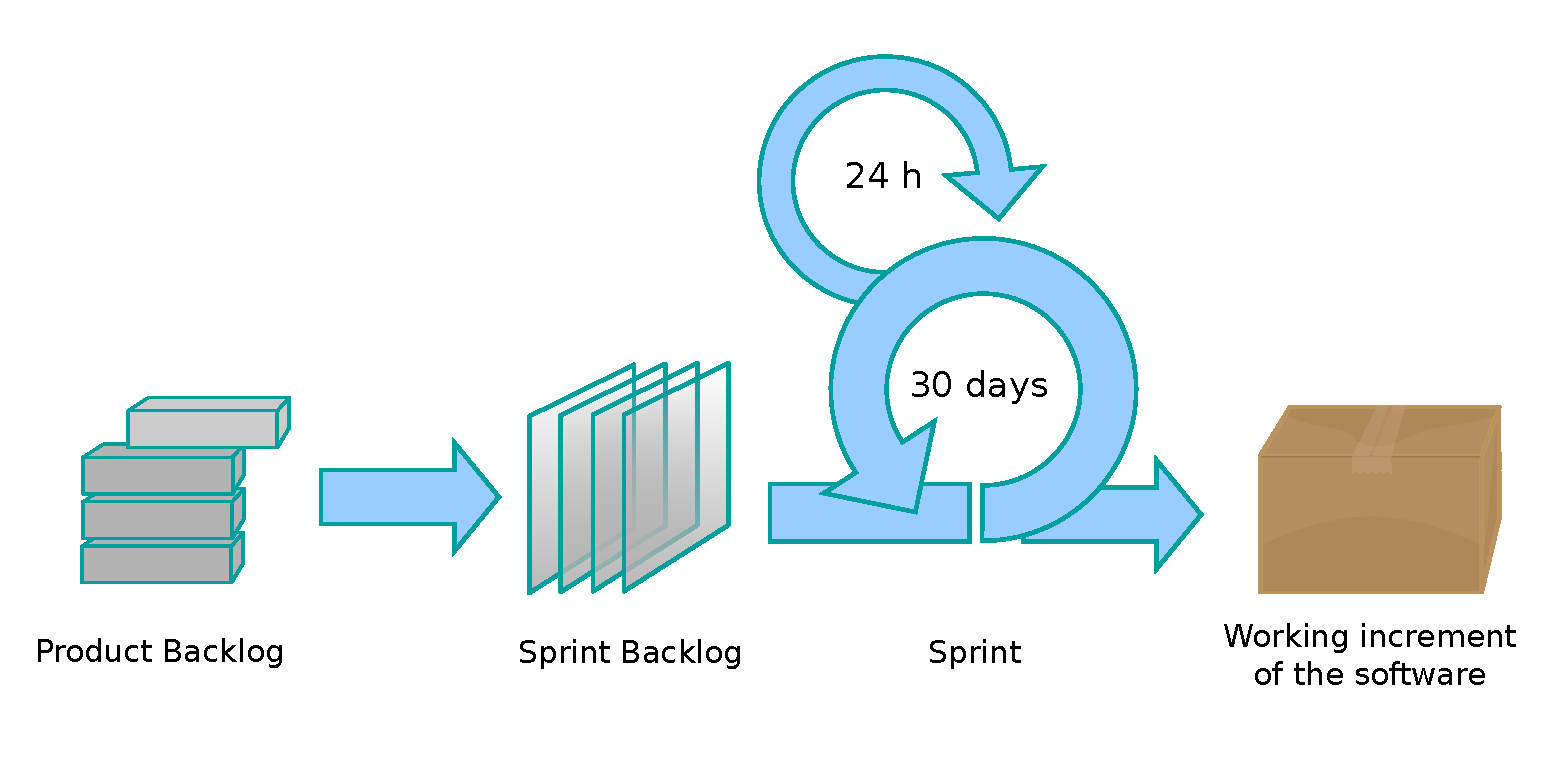
\includegraphics[scale=0.5]{swt2/scrum_process.pdf}
		\end{minipage}
	\end{itemize}
	\item \textbf{Aufgabenverteilung}
	\begin{itemize}
		\item Product Owner
		\begin{itemize}
			\item Repräsentiert den Kunden und ist für den wirtschaftlichen Erfolg des Produkts verantwortlich
			\item Erstellt/priorisiert/erklärt die Produkteigenschaften gegenüber dem Team
			\item Alleinverantwortlich für das Produkt
			\item Typische Fehler: Oft nicht verfügbar, zu wenig Durchsetzungskraft gegenüber unternehmensinternen Stakeholdern oder zu wenig technische Kenntnisse
		\end{itemize}
		\item Scrum Master
		\begin{itemize}
			\item Ist für die Umsetzung von Scrum verantwortlich
			\item Ist für die Kommunikation im Team verantwortlich
			\item Vermittelt gegenüber dem Product Owner
			\item Idealerweise ein Moderator, Coach und erfahrener Softwareentwickler
		\end{itemize}
		\item Team
		\begin{itemize}
			\item Selbstorganisierend, keine vordefinierten Rollen
			\item Idealerweise verschiedene Fachleute (GUI-Designer, Entwickler, Tester, etc.)
			\item Etwa sieben Vollzeitmitarbeiter
		\end{itemize}
		\item Kein klassischer Projektmanager vorhanden. Aufgaben werden von den drei Scrum-Rollen übernommen
	\end{itemize}
	\item \textbf{Product Backlog}
	\begin{itemize}
		\item Liste von Features, die alle Requirements beinhaltet. Nach Geschäftswert sortiert
		\item Jedes Element stellt eine User-Story da und beinhaltet eine Aufwandsangabe (\textit{Story Points})
	\end{itemize}
	\item \textbf{Sprint Backlog}
	\begin{itemize}
		\item User-Stories werden in kleinere Tasks aufgeteilt. Einzelner Task sollte nicht länger als 16 Stunden dauern
		\item Üblicherweise auf einer (non-)virtuellen Pinwand verwaltet \(\rightarrow\) bilden den Sprint Backlog
		\item Verschiedene Zustände pro Task. Beispielsweise: Todo \(\rightarrow\) In Arbeit \(\rightarrow\) Testen \(\rightarrow\) Fertig. Werden bei Zustandsänderung entsprechend verschoben/umgehängt
		\item Problem bei realen Pinwänden: Wissen geht eventuell nach Projektabschluss verloren
	\end{itemize}
	\item \textbf{Tipps für große Projekte}
	\begin{itemize}
		\item Teamgröße: Klein starten und organisch wachsen (siehe Brook's Law)
		\item Abhängigkeiten zwischen Teams verringern
		\item Daily "`Scrum of Scrums"' mit je einem (oder mehreren) Teammitgliedern
	\end{itemize}
	\item \textbf{Tipps für verteilte Teams}
	\begin{itemize}
		\item Nach Möglichkeit vermeiden
		\item Niemals Scrum Master und Team trennen
		\item Teams erst nach Eingewöhnung trennen
	\end{itemize}
\end{itemize}


\subsection{Zusammenfassung Agile Methoden}
\begin{itemize}
	\item Vorteile: Schnelles Feedback sowie reduzierte Risiken; hatte einen großen Einfluss auf Prozessverbesserung in der Industrie
	\item Nachteile: Verwenden der selben Codebasis in verschiedenen Projekten schwierig; Skalierung unklar; hoher Anspruch an die Entwickler; Dokumentation schwierig (Projekte teilweise nur im Code dokumentiert)
	\item Tendenziell Schwächen in Architektur und Design
\end{itemize}



\section{Anforderungsmanagement (Requirements Engineering)}
